\documentclass{article}
\renewcommand{\baselinestretch}{2.0} 
\usepackage{amsmath,amssymb}
\usepackage{gensymb}
\usepackage{physics}
\usepackage{graphicx}
\usepackage[a4paper, total={7in, 9in}]{geometry}
\DeclareMathSymbol{\ii}{\mathalpha}{letters}{"10}
\DeclareMathSymbol{\jj}{\mathalpha}{letters}{"11}
\newcommand{\ih}{\mathbf {\hat{\ii}}}
\newcommand{\jh}{\mathbf {\hat{\jj}}}
\newcommand{\kh}{\boldsymbol{\hat{\textbf{k}}}}
\newcommand{\rh}{\mathbf {\hat{r}}}
\newcommand{\nh}{\mathbf {\hat{n}}}
\newcommand{\ph}{\boldsymbol{\hat{\phi}}}
%\addtolength{\textheight}{+ .1\textheight}
\title{CSC 355: Compiler Design Midterm}
\author{Joy}
%\date{}
\begin{document}
\maketitle
\pagebreak
\noindent
\section*{Question 1: Reg Lang}
(a) This regular expression recognizes a language that contains strings of (ab) and (ba), that is not empty. Valid example: ab. Invalid example: $\epsilon$, $abb$
\\
(b) ... a followed by any number of a or b. Valid: a. Invalid: bb
\\
(c) ... any number of a or b that ends with abb. Valid: abb. Invalid: abbaa
\\
(d) ... any number of a followed by any number of (b then any number of a, then b, then any number of a). Valid: ababa, a. Invalid: ba, aaabababaaa
\\
(e) ... a string consisting only of a and b, that contains at least three separate substring of ``ab". Valid: ababab. Invalid: abaa
\section*{Question 2: Reg Exp}
We assume \verb|\d| is defined as \verb|0-9|.
\begin{enumerate}
  \item \verb|\(\d{3}\)\d{3}-\d{4}|
  \item We assume we want to match for both ``double varname;" and ``double varname = float;":\\ \verb|^double\s+[A-z][A-z\d_]*(\s+=\s+\d+.\d+)?;$|
  \item \verb|[ab]*babb[ab]*|
  \item Assume any year is valid, but month have to be in range (01-12), day must be in range (01-31): \\\verb!(0[1-9]|1[0-2])(\/|-)([0-2][1-9]|3[01])(\/|-)\d{2}(\d{2})?!
  \item Assume username and subdomain can be one letter: \verb|[A-z](.?[A-z\d]+)*@[A-z]+(.[A-z]+)+|
\end{enumerate}
\section*{Question 3: NFA}
(a) 
\\
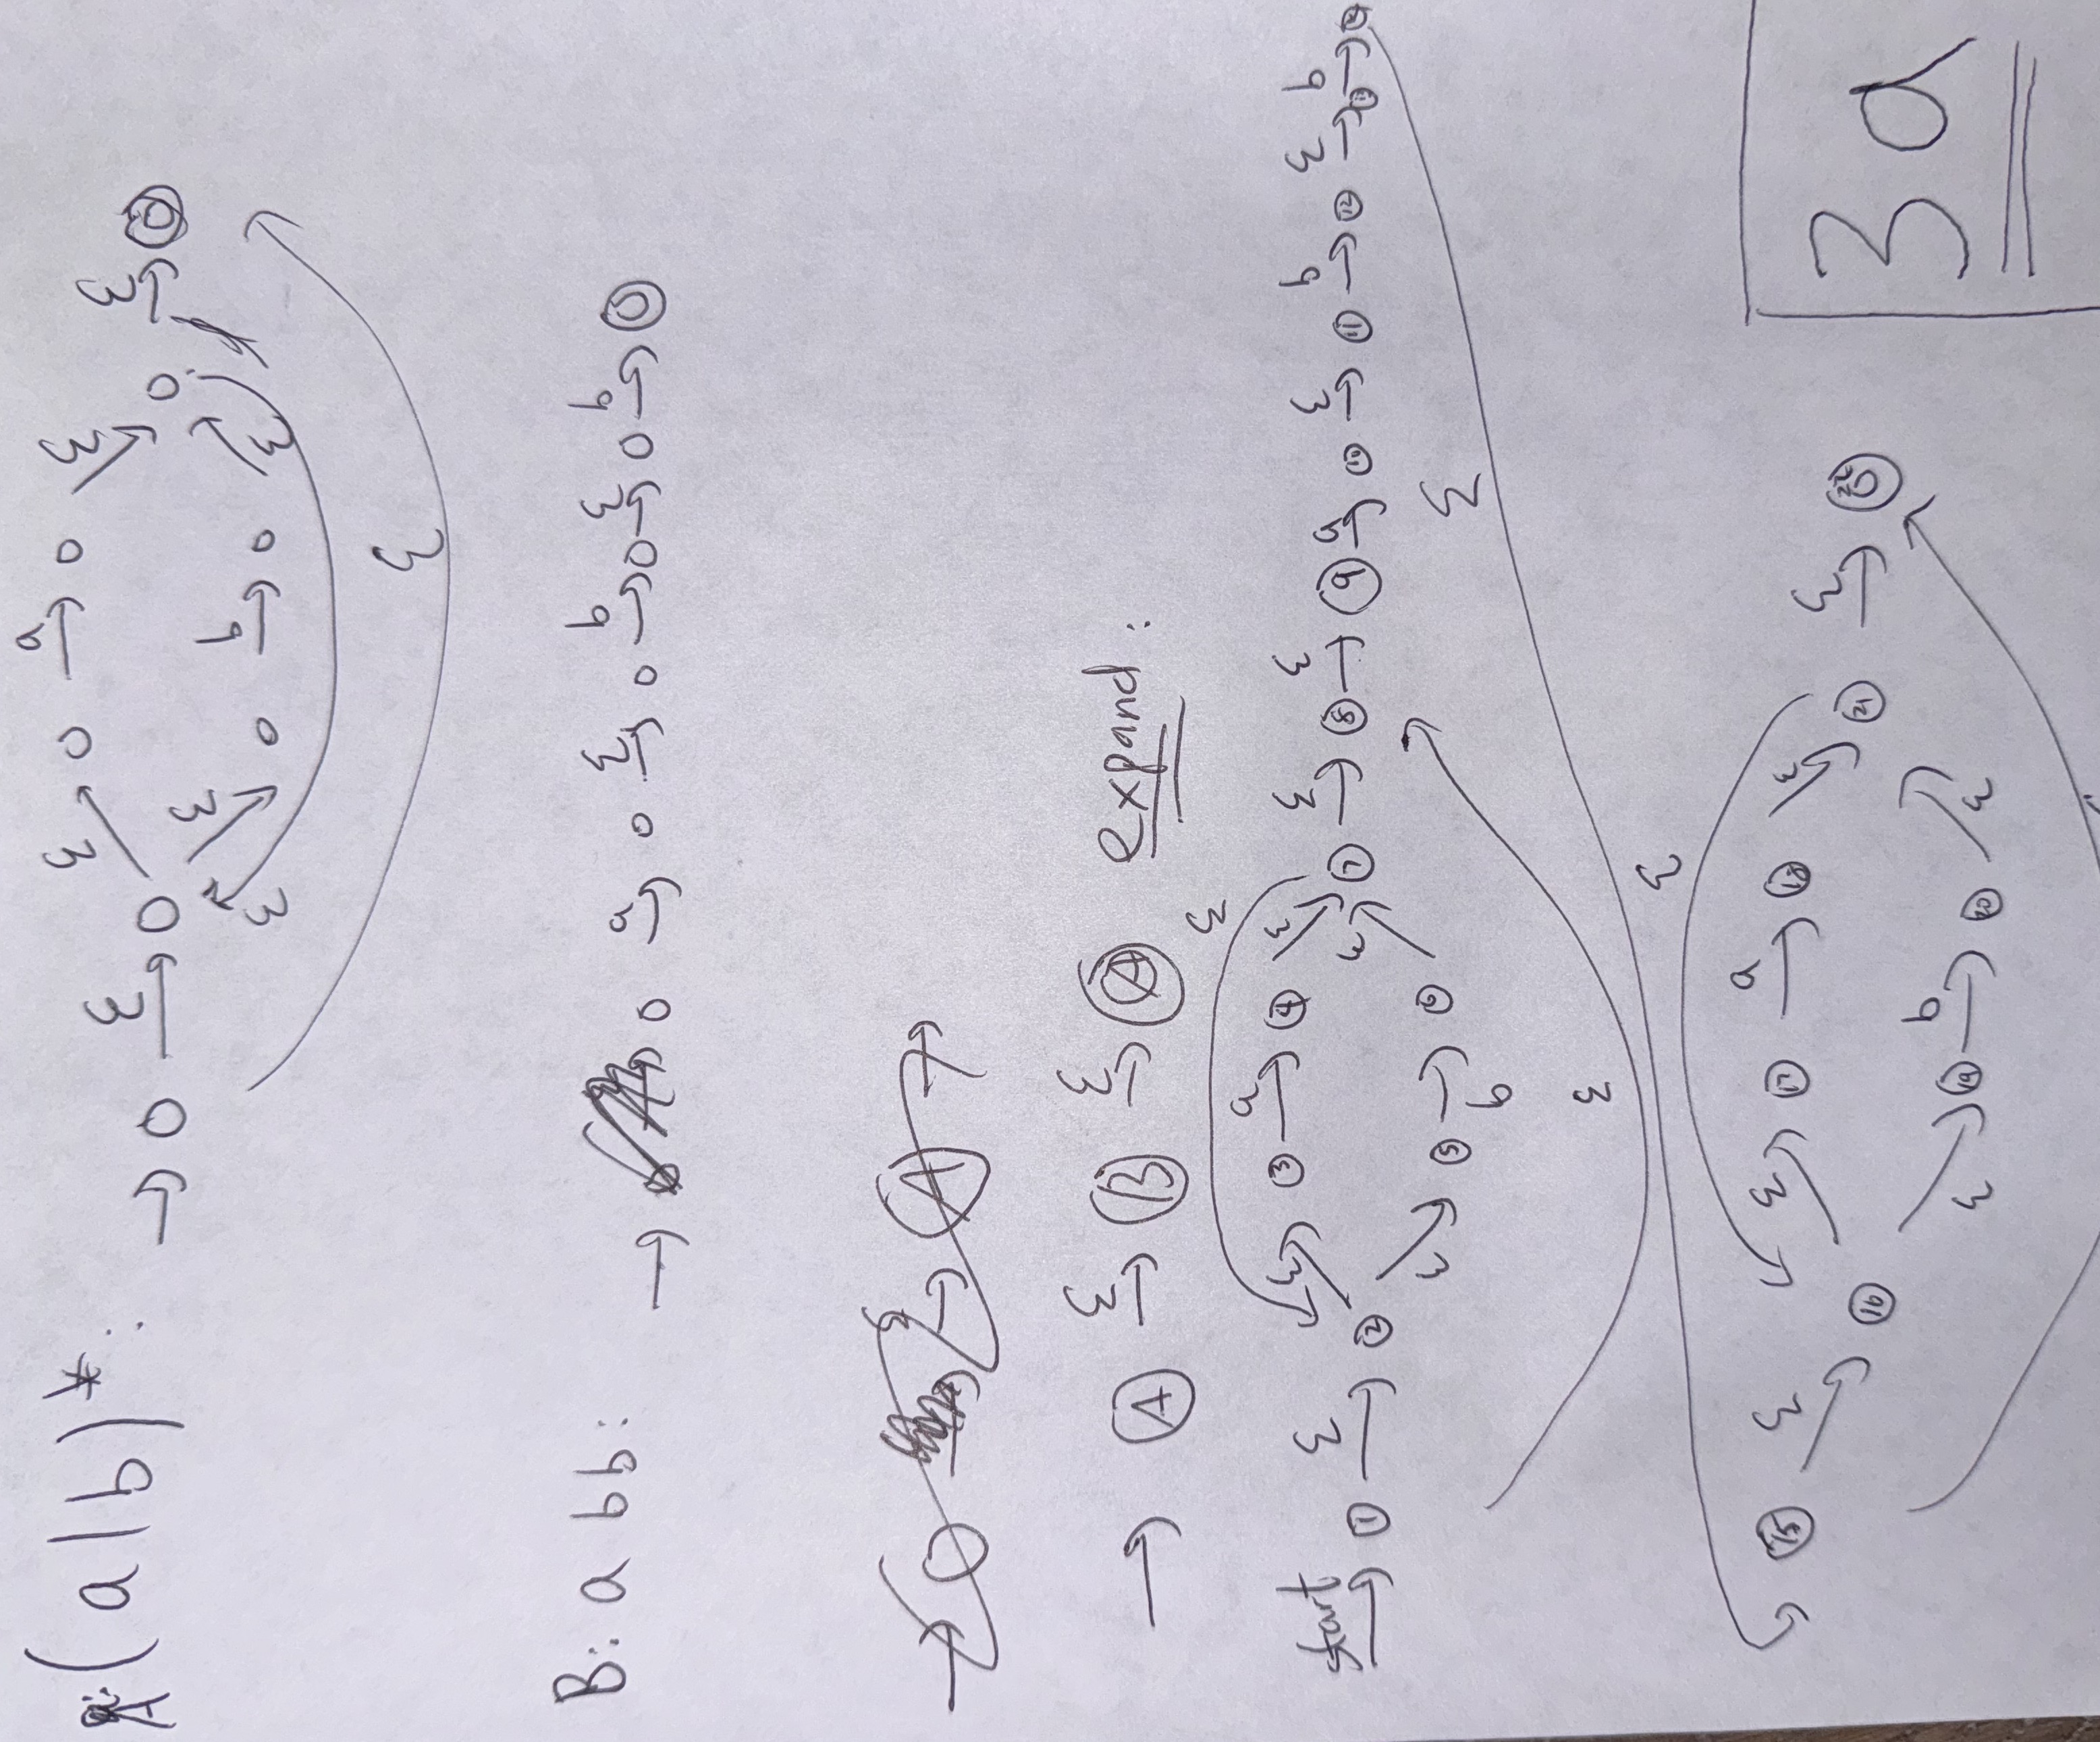
\includegraphics[angle=-90,width=\textwidth]{NFA}
\\
(b) A string made up of a or b that contains the substring of ``abb".
\\
(c) An $\epsilon$-transition is a transition between states that consume an empty string. An $\epsilon$-transition is key in MYT algo that construct a NFA by using systematic rules to synthesis base cases using concat, union, or kleenex star, because we connect these base cases with $\epsilon$-transitions. States that are connected by $\epsilon$-transition are merged into the same state in DFA (one NFA state can be merged into multiple DFA states). 
\section*{Question 4: Deterministic FA}
\begin{align}
	\epsilon\text{-closure}(1)=\{1,2,3,5,8,9\}:A
	\\
	\epsilon\text{-closure}(\text{move}(A,a))=\epsilon\text{-closure}(\{4,10\})=\{7,2,3,5,8,9,11,4,10\}:B
	\\
	\epsilon\text{-closure}(\text{move}(A,b))=\epsilon\text{-closure}(\{6\})=\{6,7,2,3,5,8,9\}:C
	\\
	\epsilon\text{-closure}(\text{move}(B,a))=\epsilon\text{-closure}(\{4, 10\})=B
	\\
	\epsilon\text{-closure}(\text{move}(B,b))=\epsilon\text{-closure}(\{6,12\})=\{6,12,7,2,3,5,13\}:D
	\\
	\epsilon\text{-closure}(\text{move}(C,a))=\epsilon\text{-closure}(\{4,10\})=B
	\\
	\epsilon\text{-closure}(\text{move}(C,b))=\epsilon\text{-closure}(\{6\})=C
	\\
	\epsilon\text{-closure}(\text{move}(D,a))=\epsilon\text{-closure}(\{4\})=C
	\\
	\epsilon\text{-closure}(\text{move}(D,b))=\epsilon\text{-closure}(\{14,6\})=\{14,6,7,2,3,5,8,9,15,16,17,19,22\}=E
	\\
	\epsilon\text{-closure}(\text{move}(E,a))=
\end{align}
I probably messed up somewhere but I did create one heuristically below.
\\\\
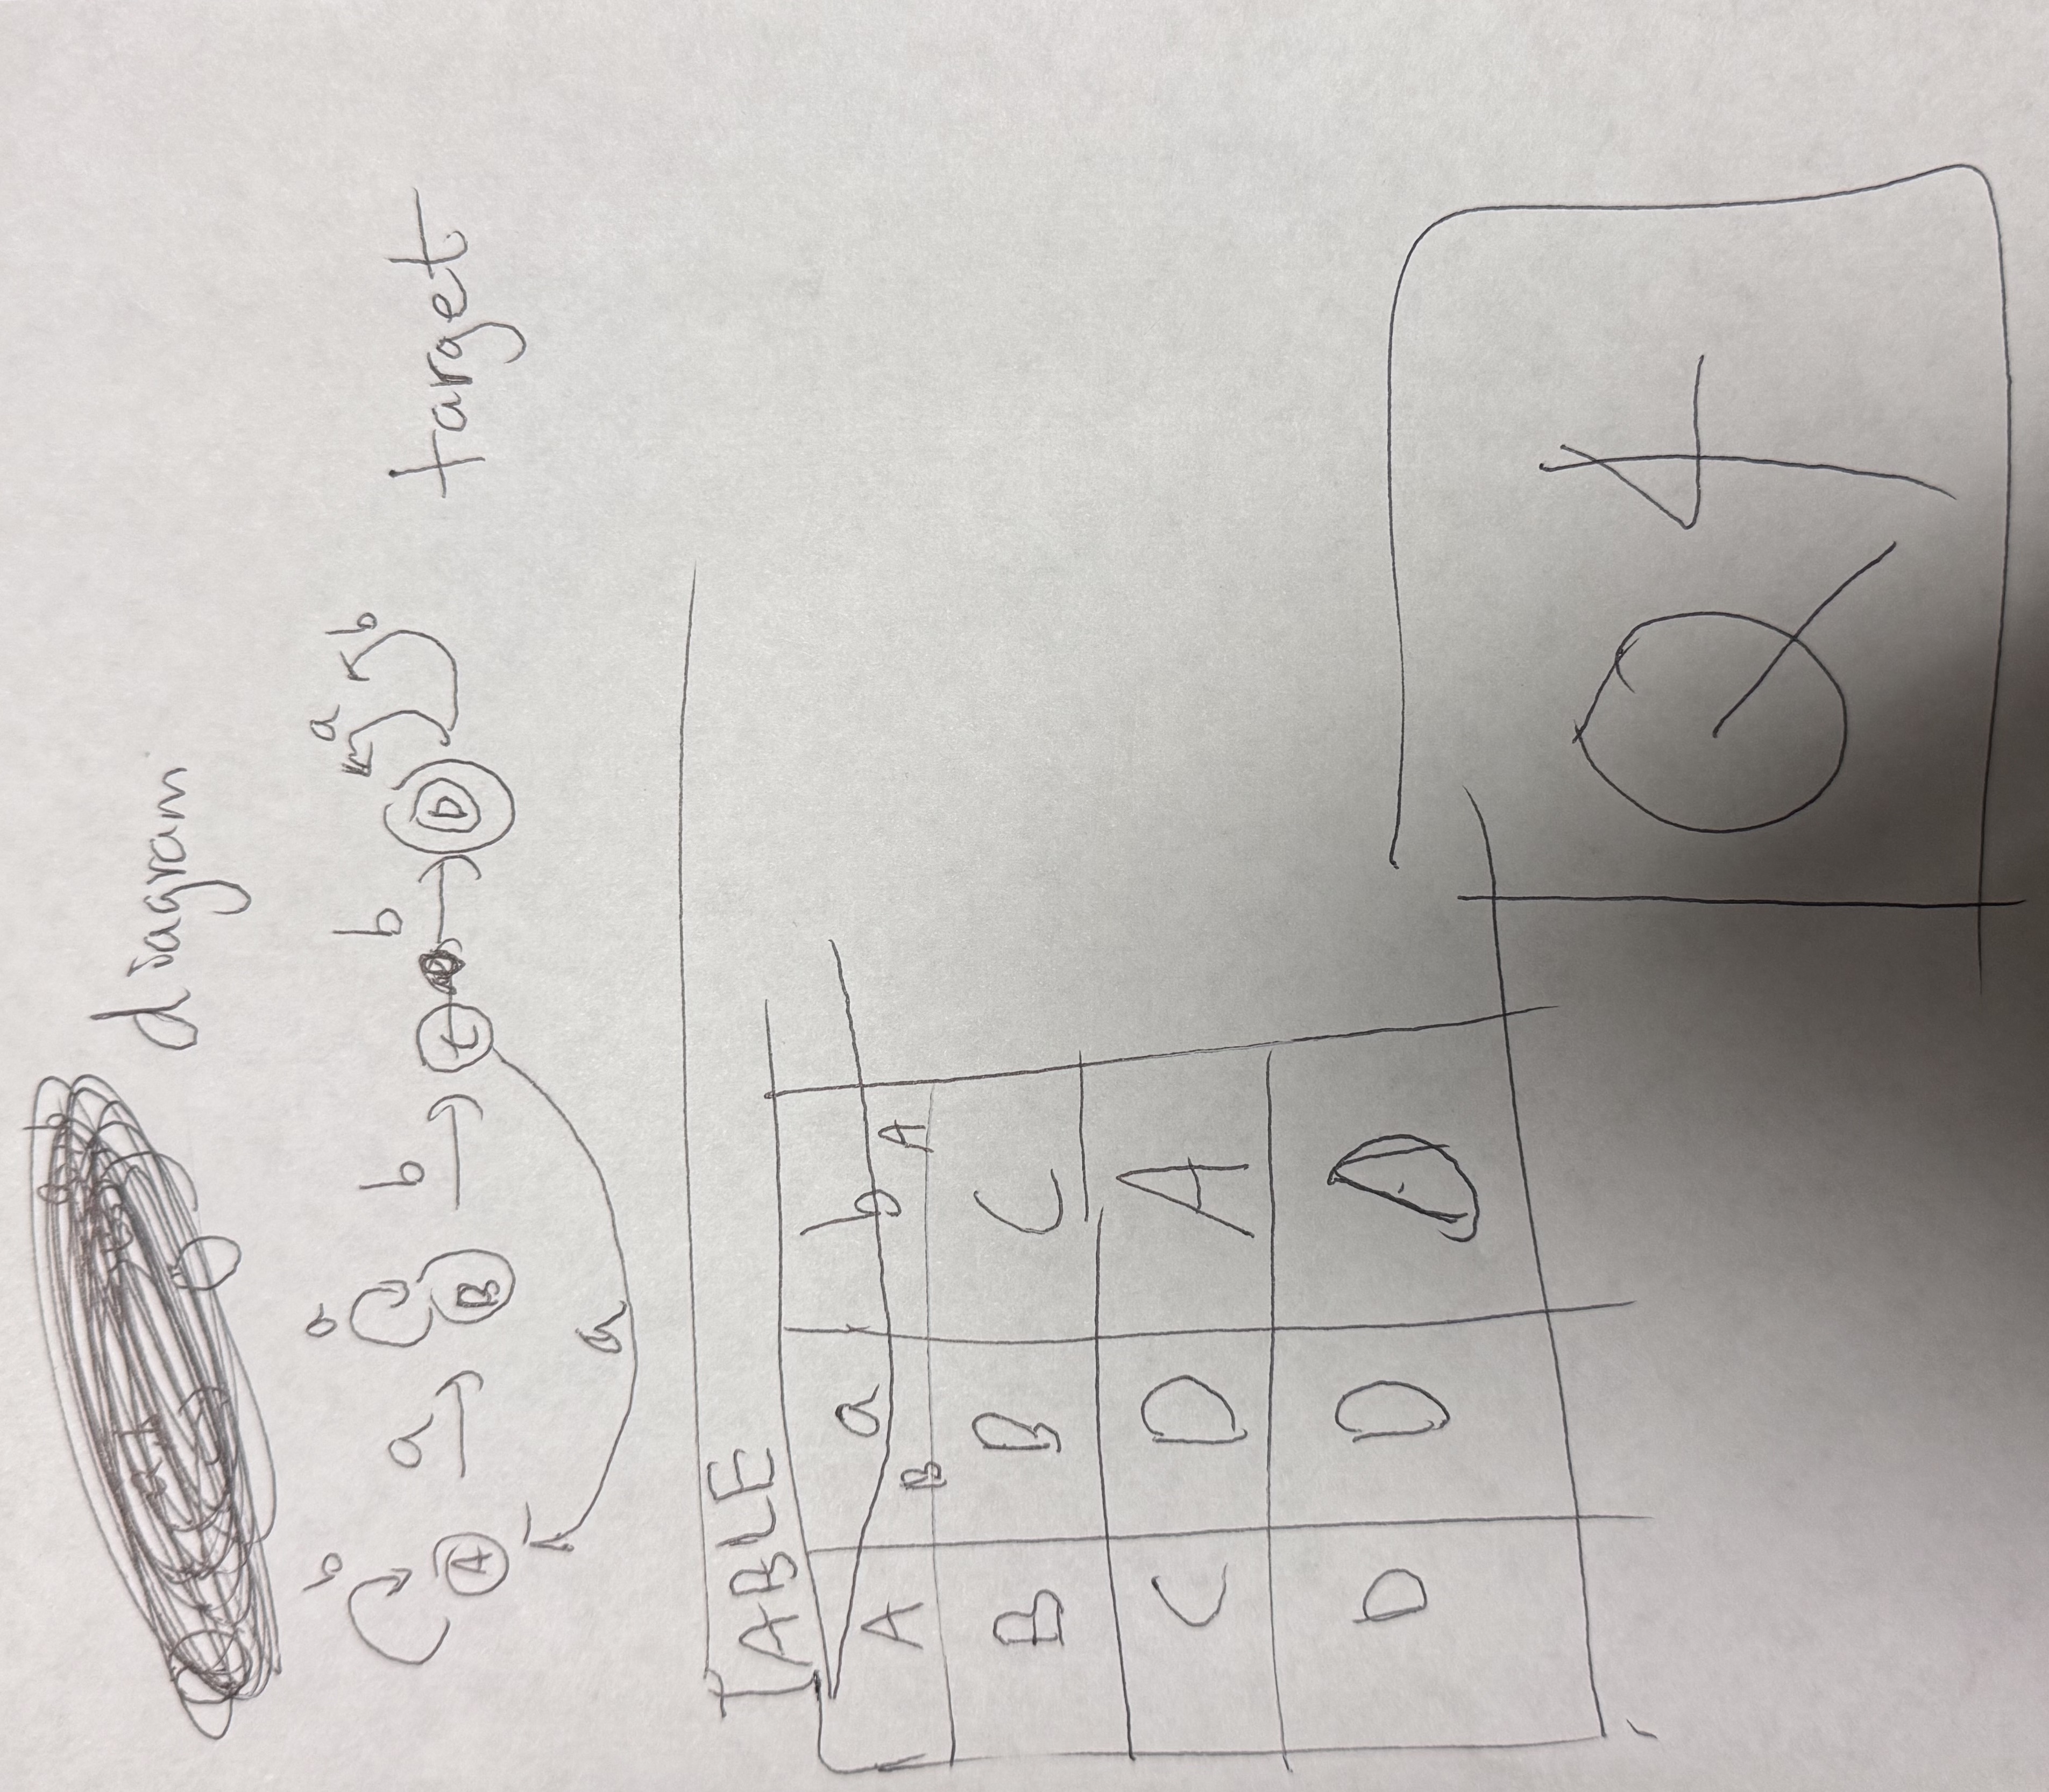
\includegraphics[angle=-90,width=\textwidth]{DFA}




\end{document}
